% Manuel de SudokuSolver (en). Compilation : python3 docs/src/compiler.py
% Préambule commun aux manuels de SudokuSolver (français et anglais), au
% format maison des PDF : Latin Modern, titres sans-serif colorés (sky pour
% les sections, alert pour les sous-sections), encadrés tcolorbox, icônes
% fontawesome, anti-titres orphelins, page de garde avec le logo.
% Compilation : python3 docs/src/compiler.py (depuis la racine du dépôt).
\documentclass[11pt,a4paper]{article}
\usepackage[utf8]{inputenc}
\usepackage[T1]{fontenc}
\usepackage{lmodern}
\usepackage{microtype}
\usepackage[a4paper,margin=2cm,headheight=24pt]{geometry}
\usepackage{graphicx}
\usepackage[table]{xcolor}
\usepackage[most]{tcolorbox}
\usepackage{enumitem}
\usepackage{booktabs}
\usepackage{array}
\usepackage{tabularx}
\usepackage[nobottomtitles*]{titlesec}
\usepackage{needspace}
\usepackage{fancyhdr}
\usepackage{fontawesome5}
\usepackage{etoolbox}
\usepackage{listings}
\usepackage{amssymb}
\usepackage[colorlinks=true,linkcolor=sky,urlcolor=sky]{hyperref}
\graphicspath{{../captures/}{../../}}
\input{version}

\definecolor{sky}{HTML}{1C6DB4}
\definecolor{skyl}{HTML}{E6F0F9}
\definecolor{alert}{HTML}{B5382B}
\definecolor{alertl}{HTML}{FBEAE8}
\definecolor{steppe}{HTML}{C08A2E}
\definecolor{steppel}{HTML}{FBF1DC}
\definecolor{summit}{HTML}{6B7A8F}
\definecolor{night}{HTML}{232A56}
\definecolor{ink}{HTML}{1F2430}
\definecolor{codegray}{HTML}{2B2B2B}
\AtBeginDocument{\color{ink}}
% Noms de couleurs de l'ancien manuel, ramenés à la palette maison
\colorlet{darkblue}{night}
\colorlet{midblue}{sky}
\colorlet{lightblue}{skyl}
\colorlet{accent}{steppe}
\definecolor{success}{HTML}{2E7D5B}
\colorlet{danger}{alert}
\definecolor{softgray}{HTML}{F6F6F6}

\titleformat{\section}
  {\Large\bfseries\sffamily\color{sky}}
  {\thesection}{0.6em}{}
  [{\vspace{1pt}\color{sky!35}\titlerule[1.3pt]}]
\titlespacing*{\section}{0pt}{16pt}{8pt}
\titleformat{\subsection}{\large\bfseries\sffamily\color{alert}}{\thesubsection}{0.5em}{}
\titlespacing*{\subsection}{0pt}{12pt}{4pt}
\titleformat{\subsubsection}{\normalsize\bfseries\sffamily\color{night}}{\thesubsubsection}{0.5em}{}
\pretocmd{\section}{\needspace{12\baselineskip}}{}{}
\pretocmd{\subsection}{\needspace{6\baselineskip}}{}{}
\widowpenalty=10000
\clubpenalty=10000
\raggedbottom
\setlength{\parindent}{0pt}
\setlength{\parskip}{6pt}
\setlist{topsep=3pt,itemsep=2pt}

\pagestyle{fancy}
\fancyhf{}
\renewcommand{\headrulewidth}{0.4pt}
\renewcommand{\headrule}{\hbox to\headwidth{\color{sky!40}\leaders\hrule height \headrulewidth\hfill}}
\fancyhead[L]{\sffamily\small\color{sky}\textbf{SudokuSolver} \color{summit}\textbar{} \MANUELTITRE}
\fancyhead[R]{\sffamily\small\color{summit}\thepage}
\fancyfoot[C]{\sffamily\scriptsize\color{summit}Version \VERSIONAPP{} \textbar{} github.com/ARP273-ROSE/SudokuSolver}

\newcommand{\menu}[1]{\textsf{\textbf{\textcolor{sky}{#1}}}}
\newcommand{\touche}[1]{\tcbox[on line,boxsep=0pt,left=2pt,right=2pt,top=1.5pt,bottom=1.5pt,
  colback=white,colframe=summit,boxrule=0.5pt,arc=1.5pt]{\footnotesize\textsf{#1}}}
\newcommand{\fichier}[1]{\texttt{\small #1}}
\newcommand{\capture}[2][1]{\par\needspace{12\baselineskip}\begin{center}\setlength{\fboxsep}{0pt}\setlength{\fboxrule}{0.6pt}%
  \fcolorbox{summit!50}{white}{\includegraphics[width=\dimexpr#1\linewidth-1.3pt\relax]{#2}}\end{center}}

% Deux captures côte à côte, chacune avec sa légende, jamais séparées
\newcommand{\deuxcaptures}[4]{\par\needspace{22\baselineskip}\begin{center}\setlength{\fboxsep}{0pt}\setlength{\fboxrule}{0.6pt}%
  \begin{minipage}[t]{0.47\linewidth}\centering\fcolorbox{summit!50}{white}{\includegraphics[width=\dimexpr\linewidth-1.3pt\relax]{#1}}\\[3pt]{\small\sffamily\color{summit}#2}\end{minipage}\hfill
  \begin{minipage}[t]{0.47\linewidth}\centering\fcolorbox{summit!50}{white}{\includegraphics[width=\dimexpr\linewidth-1.3pt\relax]{#3}}\\[3pt]{\small\sffamily\color{summit}#4}\end{minipage}\end{center}}

% Encadrés (mêmes noms et signatures que l'ancien manuel)
\newtcolorbox{infobox}[1][]{enhanced,unbreakable,colback=skyl,colframe=sky,boxrule=0.9pt,arc=2.5pt,
  left=2.5mm,right=2.5mm,top=1.5mm,bottom=1.5mm,borderline west={2.5pt}{-2.5pt}{sky},#1}
\newtcolorbox{tipbox}[2][]{enhanced,unbreakable,colback=steppel,colframe=steppe!85!black,
  coltitle=white,fonttitle=\bfseries\sffamily\small,boxrule=0.9pt,arc=2.5pt,
  left=2.5mm,right=2.5mm,top=1.5mm,bottom=1.5mm,title={\faLightbulb~~#2},#1}
\newtcolorbox{warnbox}[2][]{enhanced,unbreakable,colback=alertl,colframe=alert,
  coltitle=white,fonttitle=\bfseries\sffamily\small,boxrule=0.9pt,arc=2.5pt,
  left=2.5mm,right=2.5mm,top=1.5mm,bottom=1.5mm,title={\faExclamationTriangle~~#2},#1}

\lstset{basicstyle=\ttfamily\small\color{white},backgroundcolor=\color{codegray},
  frame=single,framerule=0pt,rulecolor=\color{codegray},xleftmargin=6pt,xrightmargin=6pt,
  framexleftmargin=6pt,framexrightmargin=6pt,aboveskip=6pt,belowskip=6pt,
  breaklines=true,showstringspaces=false,
  literate={é}{{\'e}}1 {è}{{\`e}}1 {à}{{\`a}}1 {ê}{{\^e}}1 {ç}{{\c c}}1}

\newcommand{\pagedegarde}[2]{%
  \begin{titlepage}
  \thispagestyle{empty}
  \vspace*{1.4cm}
  \begin{center}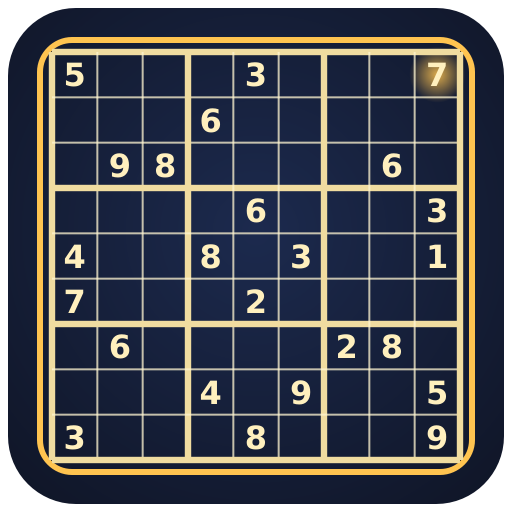
\includegraphics[width=4.4cm]{logo_512.png}\end{center}
  \vspace{8mm}
  {\sffamily\color{summit}\large SudokuSolver\par}
  \vspace{4mm}
  {\color{sky!35}\hrule height 2pt}
  \vspace{7mm}
  {\sffamily\bfseries\color{sky}\fontsize{26}{30}\selectfont #1\par}
  \vspace{4mm}
  {\sffamily\color{night}\large #2\par}
  \vspace{7mm}
  {\color{sky!35}\hrule height 2pt}
  \vspace{5mm}
  {\sffamily\color{summit}\normalsize Version \VERSIONAPP\par}
  \vfill
  {\sffamily\small\color{summit} MIT \textbar{} github.com/ARP273-ROSE/SudokuSolver\par}
  \end{titlepage}}

\usepackage[english]{babel}
\newcommand{\MANUELTITRE}{User manual}
\begin{document}
\pagedegarde{User manual}{Bilingual Sudoku solver, generator and tutor}
\tableofcontents
\newpage
% =================================================================
\section{Overview}
% =================================================================

SudokuSolver is a desktop application that solves, generates and teaches
Sudoku puzzles. It is written in Python with a PyQt6 graphical interface and
runs on Windows, Linux and macOS. The user interface is fully bilingual
(French / English) and every widget has a tooltip in both languages.

\begin{infobox}
\textbf{Key features}
\begin{itemize}
  \item Fast solver with bitmask constraint propagation and MRV backtracking
  \item 8 human-style techniques with step-by-step explanations
  \item Puzzle generator with 4 calibrated difficulty levels
  \item Interactive 9$\times$9 grid, pencil marks, real-time conflict highlighting
  \item Cross-platform (Windows, Linux, macOS)
  \item Crash reports anonymised automatically (no usernames, no paths)
\end{itemize}
\end{infobox}

% =================================================================
\section{Installation}\label{sec:en-install}
% =================================================================

\subsection{The installer (recommended)}

Ready-to-use packages, Python included, are published on the
\href{https://github.com/ARP273-ROSE/SudokuSolver/releases/latest}{releases page}.
No administrator rights are needed: everything installs into your own profile.

\begin{center}
\begin{tabularx}{\linewidth}{@{}l>{\raggedright\arraybackslash}X@{}}
\toprule
\textbf{System} & \textbf{File and first launch} \\
\midrule
Windows & \fichier{SudokuSolver-Setup.exe}. If SmartScreen warns that the
installer is unsigned: \emph{More info}, then \emph{Run anyway} (only once). \\
macOS & \fichier{SudokuSolver-X.Y.Z-macos-arm64.dmg} (Apple Silicon) or
\fichier{-macos-x86\_64.dmg} (Intel): drag the application into
Applications, then the first time \emph{right-click > Open}. \\
Linux & \fichier{SudokuSolver-X.Y.Z-linux-x86\_64.tar.gz} (or
\fichier{-linux-arm64}): unpack, then run \fichier{./installer.sh}
(installs into \fichier{\textasciitilde/.local/share}, adds the menu entry, no sudo). \\
\bottomrule
\end{tabularx}
\end{center}

This address always points at the latest Windows installer:
\begin{center}\footnotesize\url{https://github.com/ARP273-ROSE/SudokuSolver/releases/latest/download/SudokuSolver-Setup.exe}\end{center}

\subsection{Updates}

Once installed, SudokuSolver looks for a new version at start-up and on
demand (\menu{Help > Check for updates}). It downloads only the small
application archive from GitHub (any other address is refused), applies it
and restarts --- on Windows, macOS and Linux alike. The release notes are
shown in the language of the interface.

\subsection{Problem reports}

At first launch, SudokuSolver asks whether it may send a short technical
report automatically when it crashes or freezes (version, system, error
trace; nothing else). The choice can be changed at any time in the
\menu{Help} menu, where \menu{Report a problem\dots} also lets you write a
report yourself.

\subsection{Running from the sources}

Requirements: Python 3.10 or newer, \texttt{PyQt6} $\geq$ 6.5.
On Windows, \fichier{launch.bat} detects Python, creates a virtual
environment in \fichier{\%APPDATA\%\textbackslash SudokuSolver\textbackslash venv}
and starts the application; \fichier{launch.bat --repair} rebuilds it.
On Linux and macOS, \fichier{./launch.sh} does the same in
\fichier{\$XDG\_DATA\_HOME/SudokuSolver/venv}. By hand:

\begin{lstlisting}
pip install -r requirements.txt
python main.py
\end{lstlisting}

% =================================================================
\section{The interface}
% =================================================================

\subsection{Main window}

The window has four main areas:

\begin{enumerate}
  \item \textbf{Top bar} --- difficulty selector and ``New puzzle'' button.
  \item \textbf{Grid} --- the interactive 9$\times$9 board.
  \item \textbf{Action bar} --- Hint, Next step, Solve, Check, Candidates, Reset.
  \item \textbf{Explanation label} and \textbf{status bar} below.
\end{enumerate}

\deuxcaptures{en-principal.png}{The main window, with pencil marks}{en-indice.png}{A hint: the cell in green, the explanation underneath}

\subsection{Keyboard}

\begin{center}
\begin{tabular}{>{\bfseries\color{darkblue}}l l}
\rowcolor{lightblue}
Key & Action \\
\hline
Arrow keys     & Move selection \\
\rowcolor{softgray}
1--9           & Enter digit in the current cell \\
0, Delete, Backspace & Clear cell \\
\rowcolor{softgray}
Mouse click    & Select a cell \\
\end{tabular}
\end{center}

\subsection{Cell states}

\begin{itemize}
  \item \textbf{Given} --- original clue, cannot be edited, displayed in bold.
  \item \textbf{User entry} --- digit you typed, displayed in a distinct colour.
  \item \textbf{Conflict} --- cell contents violate a row, column or box rule;
        background turns red.
  \item \textbf{Candidates} --- small digits showing possible values, toggled
        by the ``Candidates'' button.
\end{itemize}

% =================================================================
\section{Features}
% =================================================================

\subsection{Generating a puzzle}

Pick a difficulty in the combo box and click \textbf{New puzzle}. The
generator creates a grid with rotational symmetry, guaranteed unique
solution, and calibrates the clue count and hardest technique required to
match the target difficulty.

\begin{center}
\begin{tabular}{>{\color{darkblue}\bfseries}l c c}
\rowcolor{lightblue}
Level   & Clues & Hardest technique \\
\hline
Easy    & 36--45 & Hidden Single \\
\rowcolor{softgray}
Medium  & 30--35 & Hidden Pair \\
Hard    & 26--32 & Box / Line Reduction \\
\rowcolor{softgray}
Expert  & 22--28 & X-Wing \\
\end{tabular}
\end{center}

Generation runs in a background thread so the interface never freezes,
even if the generator needs to retry several times to hit the target
difficulty.

\subsection{Hint}

Click \textbf{Hint} to see the next logical move. The engine picks the
simplest applicable technique, highlights the pattern cells in green and
the eliminated candidates in red, and explains \emph{why} the move works.

\begin{tipbox}{Tip}
If no technique applies, the engine falls back to a guess based on the
backtracking solver. This is very rare for generated puzzles but can
happen on imported puzzles that require advanced techniques not yet
implemented.
\end{tipbox}

\subsection{Next step}

Same as Hint, but \emph{applies} the step automatically. Chain several
``Next step'' clicks to watch the puzzle solve itself technique by
technique.

\subsection{Solve}

Fills in the complete solution instantly. The fast solver runs in a
background thread and is capped at 2\,000\,000 search nodes, which
guarantees no freeze even on pathologically hard input.

\subsection{Check}

Compares every user-entered digit against the stored solution. Wrong
cells are highlighted in red, correct cells in green. Useful when you're
not sure whether a deduction was valid.

\subsection{Candidates}

Toggles the pencil-mark display. When on, every empty cell shows its
current candidate set in small digits. When off, the cells stay clean
--- useful for a less cluttered view when you're confident about a
region.

\subsection{Reset}

Clears all user entries and restores the puzzle to its generated state.
The original clues are preserved.

\subsection{File menu}

\begin{itemize}
  \item \textbf{New} --- generate a new puzzle at the current difficulty.
  \item \textbf{Open} --- load an 81-character puzzle string from a
        \texttt{.txt} or \texttt{.sdk} file. File size is capped at 10\,KB.
  \item \textbf{Save} --- save the current grid as an 81-character string
        (dots for empty cells).
  \item \textbf{Quit} --- close the application.
\end{itemize}

\subsection{Language menu}

Switches the entire interface between French and English at once. At first
launch the language is the system's; the choice made here is remembered.

\subsection{Help menu}

\begin{itemize}
  \item \textbf{User manual (PDF)} --- this document, in the interface language (\touche{F1}).
  \item \textbf{How to play} --- a short in-app guide.
  \item \textbf{Solving techniques} --- a full bilingual catalogue of the
        8 implemented techniques (see also \fichier{guide\_techniques.pdf}).
  \item \textbf{Check for updates} --- see section~\ref{sec:en-install}.
  \item \textbf{Report a problem\dots} --- write a report, sent with the state of the grid.
  \item \textbf{Send problem reports automatically} --- the consent asked at first launch.
  \item \textbf{About} --- version and credits.
\end{itemize}

% =================================================================
\section{Under the hood}
% =================================================================

\subsection{Solver architecture}

The solver represents candidate sets as 9-bit masks (\texttt{1<<(d-1)}
for digit \texttt{d}). Every cell knows the bitwise intersection of the
allowed digits for its row, column and box. Placing a digit updates the
peers' candidate masks in constant time.

Search uses a Minimum Remaining Values (MRV) heuristic: pick the empty
cell with the fewest candidates, try each candidate in turn, propagate,
recurse. This is the same pattern used by Peter Norvig's well-known
solver, extended with an explicit node cap that bounds worst-case
effort.

\subsection{Human-style techniques}

The human solver implements eight techniques, tried in order of
increasing difficulty:

\begin{center}
\begin{tabular}{>{\color{darkblue}\bfseries}l l}
\rowcolor{lightblue}
Technique & What it finds \\
\hline
Naked Single      & Cell with only one candidate left \\
\rowcolor{softgray}
Hidden Single     & Digit that fits in only one cell of a unit \\
Naked Pair        & Two cells sharing exactly two candidates \\
\rowcolor{softgray}
Naked Triple      & Three cells sharing three candidates \\
Hidden Pair       & Two digits that fit in only the same two cells \\
\rowcolor{softgray}
Pointing Pair     & Box candidates aligned on a single row or column \\
Box/Line Reduction & Line candidates confined to one box \\
\rowcolor{softgray}
X-Wing            & 2$\times$2 rectangular elimination pattern \\
\end{tabular}
\end{center}

See \texttt{guide\_techniques.pdf} for worked examples of every
technique.

\subsection{Generator}

Generation starts from a random valid solution (shuffled backtracking),
then removes clues symmetrically while verifying after each removal that
the puzzle still has exactly one solution. The result is rated by
counting clues and running the human solver to identify the hardest
technique required. If the rating doesn't match the target difficulty,
generation retries up to 40 times before falling back to the closest
match.

\subsection{Threading and anti-freeze}

All long-running work (generation, solving) runs in dedicated
\texttt{QThread} workers. The UI thread stays responsive and the window
never freezes, even if you click ``New puzzle'' several times in a row
or import a pathologically hard grid.

Worker lifecycle is handled defensively: when a thread finishes, its
Python wrapper is cleared before Qt's native object is deleted, so
subsequent operations never touch a dangling reference.

\subsection{Crash reports}

Uncaught exceptions are caught by a \texttt{sys.excepthook} handler that
writes an anonymised JSON report (traceback, versions, system --- never the
user name nor the home folder) into the data folder, and, with your consent,
sends it to the collection point together with native crashes and interface
freezes (a watchdog notices when the window stops responding). The data
folder is outside the installation folder, which updates replace:
\fichier{\%LOCALAPPDATA\%\textbackslash SudokuSolver} on Windows,
\fichier{\textasciitilde/Library/Application Support/SudokuSolver} on macOS,
\fichier{\textasciitilde/.local/share/SudokuSolver} on Linux.

% =================================================================
\section{Troubleshooting}
% =================================================================

\subsection{``Python not found'' on Windows}

The launcher couldn't find a working Python interpreter. Install
Python 3.10 or newer from \url{https://www.python.org/downloads/} and
\textbf{make sure to tick ``Add Python to PATH''} during installation.
Then re-run \texttt{launch.bat}.

\subsection{``Installation failed'' after a Python upgrade}

If you upgraded Python and the old venv is stale, run:

\begin{lstlisting}
launch.bat --repair
\end{lstlisting}

This deletes the virtual environment and reinstalls everything cleanly.

\subsection{The generator is slow on Expert}

Expert puzzles that specifically require X-Wing are rare, so the
generator may retry up to 40 times before falling back to a Hard-level
puzzle with a slightly more constrained clue count. This is by design,
and the background thread keeps the UI responsive throughout.

\subsection{I imported a puzzle and Solve says ``no solution''}

Either the imported grid has a typo (wrong digit in a given), it
already contains a conflict (check the red highlights), or it genuinely
has no solution. The solver also bails out after 2\,000\,000 search
nodes --- this almost never triggers on valid 9$\times$9 grids.

\subsection{Where are my settings stored?}

The only setting, the language, is kept by Qt in the user's preferences
(registry on Windows, \fichier{\textasciitilde/.config} on Linux, preferences
on macOS). The log and the reports live in the data folder described in the
\emph{Crash reports} section; nothing is written into the installation
folder.

\subsection{The app crashed --- what should I do?}

If you accepted automatic reports, there is nothing to do: the report has
been sent. Otherwise, use \menu{Help > Report a problem\dots} and describe what
you were doing; without a connection, the report is saved as a \fichier{.zip}
on the desktop, ready to be attached to a GitHub issue.

% =================================================================
\section{FAQ}
% =================================================================

\subsubsection*{Can I play on a phone?}
No --- this is a desktop application. For mobile, use any Sudoku app
from your platform's store.

\subsubsection*{Does it phone home?}
Only for two things: the update check (GitHub releases API, once at
start-up) and, if you agreed, problem reports. No analytics, no grid data
unless you send a written report.

\subsubsection*{What Sudoku formats are supported?}
81-character strings with digits \texttt{1--9} and any of \texttt{.},
\texttt{0}, \texttt{-} or space for empty cells. Line breaks are
tolerated.

\subsubsection*{Why is the ``Solving techniques'' guide a separate PDF?}
Because it is a reference you want to browse while solving. The main
manual (this document) is the ``how to use the app'' guide; the
techniques guide is the ``how to solve Sudoku'' reference.

% =================================================================
\section{Credits}
% =================================================================

SudokuSolver is MIT-licensed. Thanks to Peter Norvig for the classic
constraint-propagation solver design, and to the Sudoku solving
community for decades of accumulated technique catalogues.

\medskip
Issues and contributions welcome at:\\
\url{https://github.com/ARP273-ROSE/SudokuSolver}
\end{document}
